% !TEX root = Dokumentation.tex
\subsection{Risikomanagement}
Die Risiken, die während der Projektdurchführung entstehen könnten, sind im Folgenden aufgelistet. Um zu wissen, wie hoch ein Risiko eingeschätzt werden muss wurde eine Grafik erstellt. Zu jedem Risiko sind auch Massnhamen aufgelistet, welche im Eintrittsfall unternommen werden können. \\

\begin{figure}[H]%Position festigen
\centering
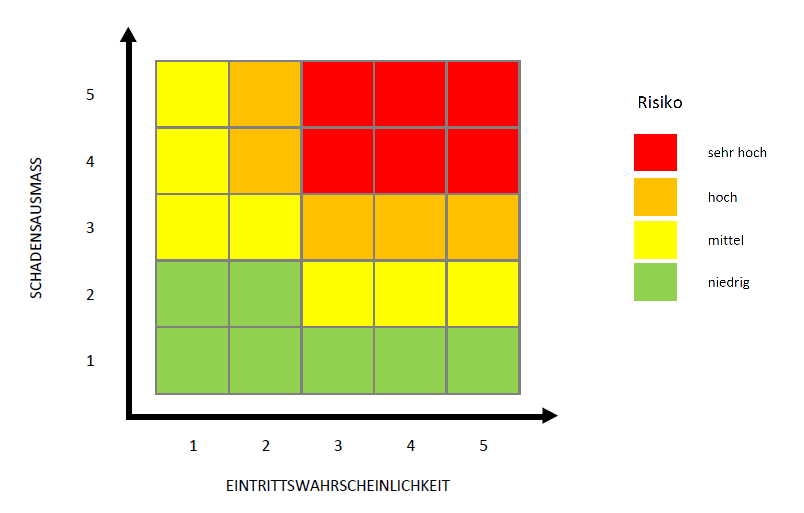
\includegraphics[width=0.8\textwidth]{Images/risikomatrix.png}
\caption{Risikomatrix}
\label{fig:Risikomatrix}
\end{figure}

\subsubsection{Risiken im Team}
\begin{table}[H]
\begin{tabular}{|p{0.3\textwidth}|p{0.2\textwidth}|p{0.2\textwidth}|p{0.2\textwidth}|}\hline
	
	\textbf{Risiko}	& 	\textbf{Wahrscheinlichkeit} & \textbf{Schadensausmass}  & \textbf{Massnahmen} \\\hline
	

	Mitglied verlässt das Team	&	1	&	4	&	Neuverteilung der Arbeiten \\\hline
	Unzuverlässigkeit eines Teammitglieds	&	2	&	3-4	&	 Absprache im Team, um eine Lösung zu finden  \\\hline
	Unstimmigkeiten unter den Teammitgliedern	& 	3	&	4	& Absprache im Team, um eine Lösung zu finden, evtl. auch Rat von Supervisor einholen.  \\\hline
	Mitglied überlastet	&	4	&	3	&	Neuverteilung der Arbeiten \\\hline
	Kommunikations-probleme	&	4	&	3	&	verbessert Absprachen, Frequenz der Sitzungen erhöhen \\\hline
	Fehlende fachliche Kompetenz eines Mitglieds	&	2	&	2	&	Neuverteilung der Arbeiten \\\hline
	Fehlende soziale Kompetenz eines Mitglieds	&	1	&	3	&	Absprache im Team, um eine Lösung zu finden \\\hline
\end{tabular}\\
\end{table}

\subsubsection{Risiken Projektmanagement}
\begin{table}[H]
\begin{tabular}{|p{0.3\textwidth}|p{0.2\textwidth}|p{0.2\textwidth}|p{0.2\textwidth}|}\hline
	
	\textbf{Risiko}	& 	\textbf{Wahrscheinlichkeit} & \textbf{Schadensausmass}  & \textbf{Massnahmen} \\\hline
		Missverständnisse bei den Anforderungen	&	3-4	&	3	& Absprache mit Supervisor  \\\hline
	Ineffizientes Arbeiten	&	3-4	&	2-3	& Neuorganisierung der Vorgehensweise  \\\hline
	
	Überschreitung des Budgets	&	1	&	4	& Absprache mit Supervisor  \\\hline
\end{tabular}\\
\end{table}

\subsubsection{Risiken bei der Realisierung}
\begin{table}[H]
\begin{tabular}{|p{0.3\textwidth}|p{0.2\textwidth}|p{0.2\textwidth}|p{0.2\textwidth}|}\hline
	
	\textbf{Risiko}	& 	\textbf{Wahrscheinlichkeit} & \textbf{Schadensausmass}  & \textbf{Massnahmen} \\\hline
	
	Idee funktioniert nicht wie gewünscht	&	2	&	4 & neue Ideenfindung, Rat einholen  \\\hline
	Eingekaufte Komponente erfüllt Anforderung nicht	&	2	&	5	& andere Komponente einkaufen  \\\hline
		Projekt-anforderungen sind nicht erfüllt	&	1	&	5	&  Anpassungen planen \\\hline
\end{tabular}\\
\end{table}

\subsubsection{Andere Risiken}
\begin{table}[H]
\begin{tabular}{|p{0.3\textwidth}|p{0.2\textwidth}|p{0.2\textwidth}|p{0.2\textwidth}|}\hline
	
	\textbf{Risiko}	& 	\textbf{Wahrscheinlichkeit} & \textbf{Schadensausmass}  & \textbf{Massnahmen} \\\hline
	
	Lange Lieferzeiten bei Bestellungen	&	3	&	2	& andere Arbeiten aufnehmen, früher bestellen  \\\hline
	Github fällt aus	&	1	&	4	& Lokal weiterarbeiten  \\\hline
\end{tabular}\\
\end{table}

